% !TEX TS-program = pdflatex
% !TEX root = ../LightMicroRep.tex

%************************************************
\chapter{Expansion Microscopy}
\label{chp:Expansion}
%************************************************
%\numberwithin{figure}{section}
%----------------------------------------------------------------------------------------
%	INTRODUCTION
%----------------------------------------------------------------------------------------

\section{Introduction}

\paragraph{Aim} To enlarge a specimen by following an expansion microscopy protocoll.
\\

Expansion microscopy utilize a non-traditional approach to obtain a high resolution images. 
Instead of relying on state of the art devices to observe minute structures, this approach aims to magnify/expand the specimen itself and allows the observation to be conducted , in principle, using a conventional diffraction-limited microscopes. 
The use of a high resolution microscope would allow an even better observation. 
This expansion is achieved by means of linking a stained sample to a gel matrix that swells by absorbing water. 
The general scheme is shown in Fig. ~\ref{fig:exmgensch}.

\begin{figure}[h!]
\centering
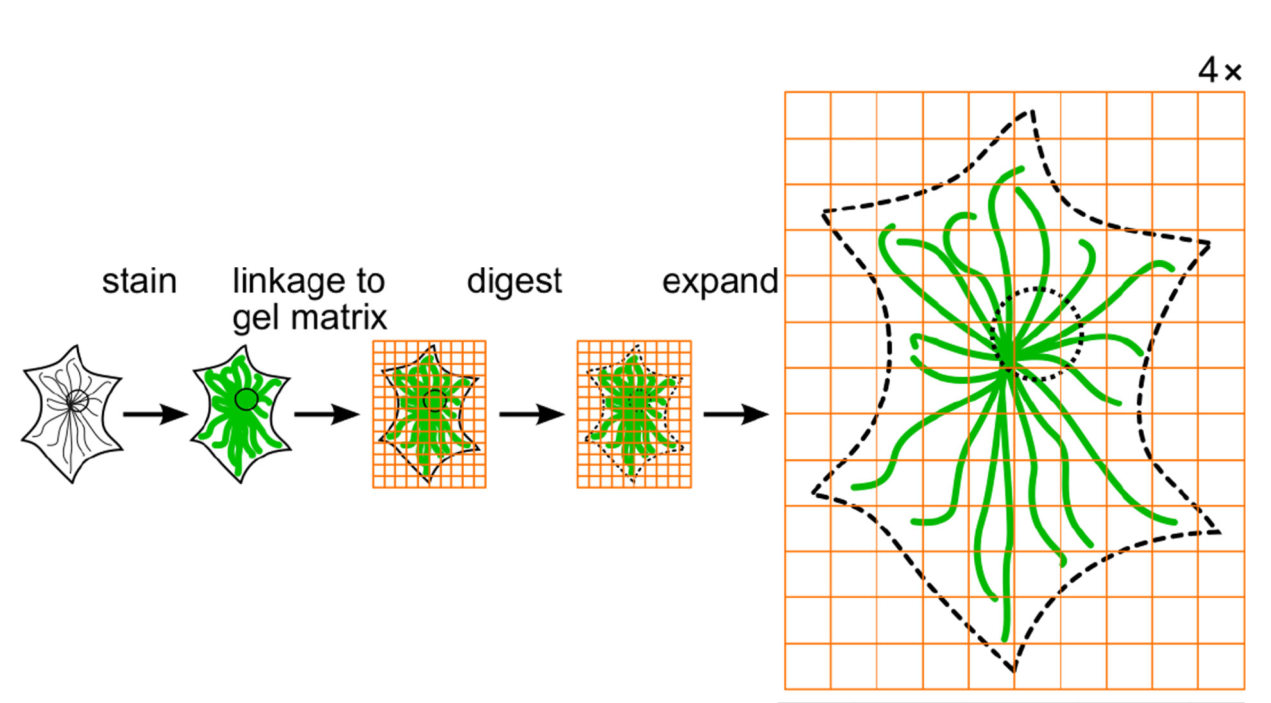
\includegraphics[width=.6\columnwidth]{Exp_5_Expansion/Figures/genscheme}
\caption{General scheme of expansion microscopy. Image adapted from Chen et al \cite{Chen2015}.} 
\label{fig:exmgensch}
\end{figure}
%----------------------------------------------------------------------------------------
%	METHODS
%----------------------------------------------------------------------------------------
\section{Methods}

Two samples of the AX2 line of \textit{Dictyostelium discoideum} was stained, embedded to polymer matrix, digested, and expanded according to protocol (also made is a non-expanded control).  
The centrosome core (CP91) is labelled by AlexaFluor568 (red), the corona of the centrosome (CP224) by AlexaFluor488 (green), and nucleus is by DAPI (blue).

%----------------------------------------------------------------------------------------
%	RESULTS AND DISCUSSION
%----------------------------------------------------------------------------------------
\section{Results and Discussion}

The calculation result of the expansion procedure of the gel matrix is shown in Fig.~\ref{fig:matarea}. 
As can be seen here, the expansion process succeeds in enlarging the gel matrix to more than 4 times the original size, and consequently, the cells embedded inside as well.  

The resulting sample is then imaged by LSM, shown in Fig.~\ref{fig:axexp}. 
As can be inspected here, the resolution is increased dramatically. 
Comparison between Fig~\ref{NEr} to Fig~\ref{Er} show that CP91 can be seen with a more prominent structure post-expansion. 
This is also the case in Fig~\ref{Eg} where it can be observed that CP224 can be imaged showing more features instead of just a bright dot like in Fig~\ref{NEg}. 
It can also be seen a lot clearer here that the fluorescence label AlexaFluor488 sticking to the $+$ ends of microtubules whereas in the control image these features are observable as a hazy cloud. 
The nucleus that is shown as being only a blurry cloud in Fig~\ref{NEb} can now be imaged with a much higher resolution as seen in Fig~\ref{Eb}.

\begin{figure}
\begin{minipage}[m]{0.33\columnwidth}
\vspace{10mm}
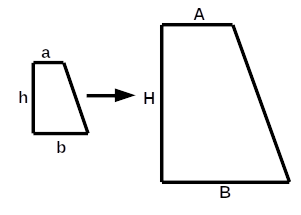
\includegraphics[width=.9\columnwidth]{Exp_5_Expansion/Figures/trapeth}
\end{minipage}
\begin{minipage}[b]{0.55\columnwidth}
\centering
\begin{tabular}[m]{cllc}
\toprule
& \thead{Pre-Expansion\\(cm)} & \thead{Post-Expansion\\(cm)} & \thead{Enlargement\\Factor}\\
\midrule
\thead{Sample 1}	&\thead[l]{a: 0.45\\b: 0.60\\h: 0.75\\Area: 0.39}&\thead[l]{A: 1.50\\B: 2.70\\H: 3.30\\Area: 6.93}& \texttildelow4.2$\times$\\
\thead{Sample 2}	&\thead[l]{a: 0.65\\b: 0.80\\h: 0.75\\Area: 0.54}&\thead[l]{A: 2.50\\B: 3.40\\H: 3.40\\Area: 10.03}& \texttildelow4.3$\times$\\		
\bottomrule
\end{tabular}
\end{minipage}
\caption{\textbf{Left}: Schematic of the dimension of pre- and post-expansion gel matrix. 
\textbf{Right}: Table of measurement details (pre- and post-expansion) of both samples, including the the area and enlargement factor.}
\label{fig:matarea}
\end{figure}

\begin{figure}[h]
\centering
\captionsetup[subfigure]{position=top}
\subfloat[Control\label{NEc}]{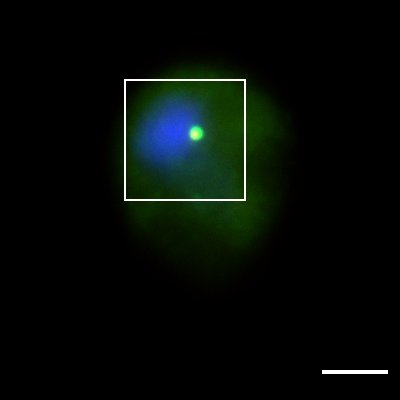
\includegraphics[width=.23\columnwidth]{Exp_5_Expansion/Figures/bNExpComp_3um}}\hspace{0.1mm}
\subfloat[CP91\label{NEr}]{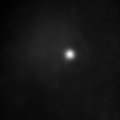
\includegraphics[width=.23\columnwidth]{Exp_5_Expansion/Figures/bNExpred}}\hspace{0.1mm}
\subfloat[CP224\label{NEg}]{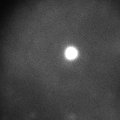
\includegraphics[width=.23\columnwidth]{Exp_5_Expansion/Figures/bNExpgreen}}\hspace{0.1mm}
\subfloat[Nucleus\label{NEb}]{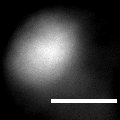
\includegraphics[width=.23\columnwidth]{Exp_5_Expansion/Figures/bNExpblue_3um}}\vspace{-0.7em}
\captionsetup[subfigure]{position=bottom}
\subfloat[Expanded\label{Ec}]{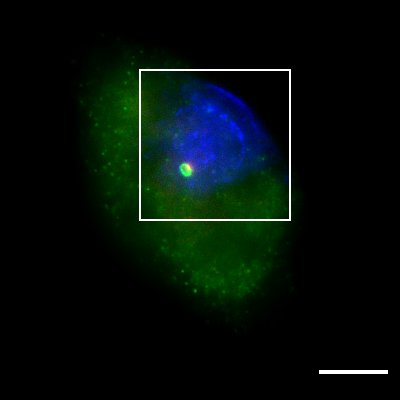
\includegraphics[width=.23\columnwidth]{Exp_5_Expansion/Figures/bExComp_10um}}\hspace{0.1mm}
\subfloat[Exp. CP91\label{Er}]{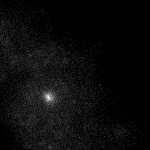
\includegraphics[width=.23\columnwidth]{Exp_5_Expansion/Figures/bExred}}\hspace{0.1mm}
\subfloat[Exp. CP224\label{Eg}]{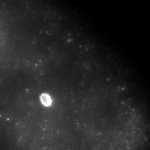
\includegraphics[width=.23\columnwidth]{Exp_5_Expansion/Figures/bExgreen}}\hspace{0.1mm}
\subfloat[Exp. Nucleus\label{Eb}]{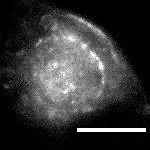
\includegraphics[width=.23\columnwidth]{Exp_5_Expansion/Figures/bExblue_10um}}\\
\caption{AX2 specimen composite and the magnified channel breakdown. 
White squares mark the magnified areas of images on the right of the composite. 
Control specimen at top row and expanded at bottom row. 
Shown here are single representative optical sections of a z-stack. 
Objective lens: Plan-Apochromat 100$\times$/1.40 Ph3 oil immersion (control) and LCI Plan-Neofluar 63$\times$/1.30 Imm Korr DIC water immersion (expanded). 
Scalebars are 3 $\mu$m for the control (both original and magnified images) and 10 $\mu$m for the expanded (both). 
Gamma correction of 1.50 was applied for all images.} 
\label{fig:axexp}
\end{figure}


%----------------------------------------------------------------------------------------
%	BIBLIOGRAPHY
%----------------------------------------------------------------------------------------

\renewcommand{\refname}{\spacedlowsmallcaps{References}} % For modifying the bibliography heading

%\bibliographystyle{unsrt}

%\bibliography{sample.bib} % The file containing the bibliography
